% *******************************************************************************
% * Copyright (c) 2007 by Elexis
% * All rights reserved. This document and the accompanying materials
% * are made available under the terms of the Eclipse Public License v1.0
% * which accompanies this distribution, and is available at
% * http://www.eclipse.org/legal/epl-v10.html
% *
% * Contributors:
% *    G. Weirich - initial implementation
% *
% *  $Id: konsviews.tex 2453 2007-05-30 15:16:13Z rgw_ch $
% *******************************************************************************
% !Mode:: "TeX:UTF-8" (encoding info for WinEdt)


\section{Konsultationsbezogene Views}

\subsection{Fälle}
Diese View (Abb. \ref{fig:faelle} listet alle für den aktuell selektierten
Patienten existierenden Fälle. \index{Fall-Liste}
\begin{figure}[htp]
\begin{center}
  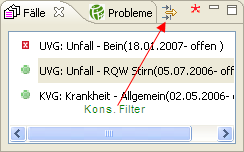
\includegraphics{images/faelleview}
  \caption{Fälle - View}
  \label{fig:faelle}
\end{center}
\end{figure}

Das Symbol links von der Fallbezeichnung gibt an, ob alle für die Verrechnung
des Falles notwendigen Daten vorhanden sind: Wenn es grün ist, sollte die
Rechnungserstellung möglich sein, wenn es rot ist, fehlen noch eine oder mehrere
Angaben. \textit{Welche} Angaben mindestens notwendig sind, hängt von der Art
des Falles ab. So ist für Fälle, die nach dem KVG abgerechnet werden, die Angabe
eines Rechnungsempfängers, eines Versicherers und der Versichertennummer
notwendig. Bei Fällen, die nach UVG abgerechnet werden, muss eine Fallnummer
vorhanden sein.

Rechtsklick auf einen Fall öffnet dessen Kontextmenü. Dieses enthält die
folgenden Punkte:
\begin{itemize}
  \item {Fall löschen}. Dies ist nur möglich, wenn Sie die dazu notwendigen Rechte
  haben, und wenn zu diesem Fall keine Konsultationen mehr existieren.
  \item {Fall bearbeiten}. Dies öffnet eine weitere View, in der Details zum
  aktuell ausgewählten Fall eingegeben werden können.
  \item {Fall wieder öffnen}. Damit kann man einen bereits
  geschlossenen\footnote{Ein Fall ist dann geschlossen, wenn ein End-Datum
  eingegeben wurde. Zu einem geschlossenen Fall können keine Konsultationen mehr
  hinzugefügt werden.} Fall wieder öffnen.
  \item {Rechnung erstellen}. Hiermit lässt sich über alle unverrechneten
  Konsultationen des aktuellen Falls und des aktuellen Mandanten eine Rechnung
  erstellen. Dies ist eine \glqq Abkürzung\grqq{} des normalen Wegs der
  Rechnungserstellung und eignet sich vor allem für Sofortrechnungen einzelner
  Konsultationen oder Leistungen.
\end{itemize}
\subsection{Fälle und Kons}
Diese View (Abb. \ref{fig:fallkons} listet synoptisch Fälle und dazugehörige
Konsultationen (Nur Titel ohne Texte) auf. Wenn im oberen Bereich ein Fall
angeklickt wird, werden im unteren Bereich die zu diesem Fall gehörenden
Konsultationen angezeigt. Wenn eine Konsultation angeklickt wird, wird diese
Konsultation in der Konsultation-View (S. s. \pageref{konsview}) angezeigt.

 %\usepackage{graphics} is needed for \includegraphics
\begin{figure}[htp]
\begin{center}
  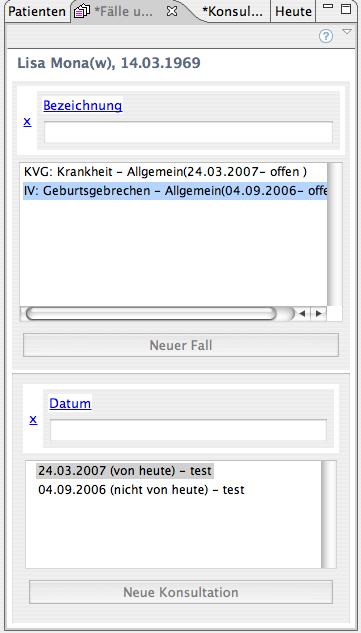
\includegraphics{images/fallkonsview}
  \caption{Fälle und Kons}
  \label{fig:fallkons}
\end{center}
\end{figure}

\subsection{Konsultationen}
Dies ist eine Auflistung aller bisherigen Konsultationen des aktuell
selektierten Patienten, unabhängig vom jeweiligen Fall.
\index{Konsultationsliste} Zu jeder Konsultation
wird der Text ohne Formatierungen angezeigt. (S. Abb. \ref{fig:konslisteview}).
%\usepackage{graphics} is needed for \includegraphics
\begin{figure}[htp]
\begin{center}
  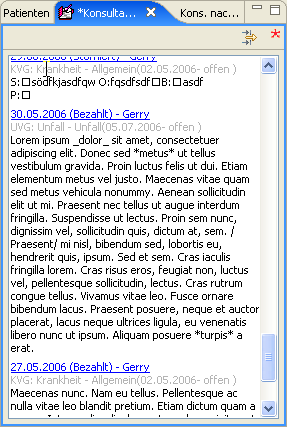
\includegraphics{images/konslisteview}
  \caption{Konsultationsliste}
  \label{fig:konslisteview}
\end{center}
\end{figure}
Klick auf den (blauen) Titel einer Konsultation wählt diese Konsultation in der
Konsultation-View (s. S. \pageref{konsview}) aus.

Klick auf das Filter-Symbol rechts oben öffnet den Filter-Dialog (s. Abb. \ref{fig:konsfilter}).
\begin{figure}[htp]
\begin{center}
  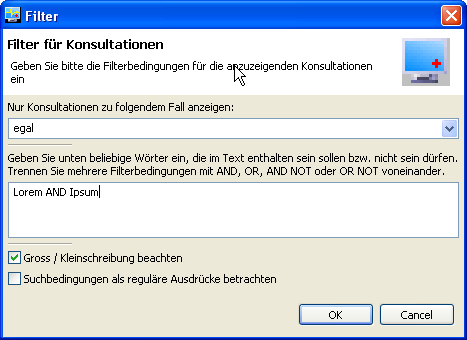
\includegraphics{images/filterdialog}
  \caption{Filterdialog}
  \label{fig:konsfilter}
\end{center}
\end{figure}
\index{Konsultationsfilter} Hier können Sie bestimmte Kriterien eingeben, nach
denen die angezeigten Konsultationen gefiltert werden sollen (d.h. es werden nur
noch diejenigen Konsultationen angezeigt, die den Filterbedingungen
entsprechen).

Im Oberen Feld können Sie angeben, ob nur Konsultationen eines bestimmten Falls
oder aller Fälle angezeigt werden sollen. Im unteren Feld können Sie
Suchbegriffe eingeben, welche im Konsultationstext vorkommen müssen. Mehrere
Suchbegriffe können mit AND, OR, NOT, AND NOT und OR NOT miteinander verknüpft werden.
Beispielsweise findet \glqq Lorem AND NOT ipsum\grqq{} nur solche Konsultationen, deren
Text \glqq Lorem\grqq, nicht aber \glqq ipsum\grqq{}enthält.

Ganz unten können Sie schliesslich noch angeben, ob Gross/Kleinschreibung
beachtet werden soll, oder ob Suchbegriffe als reguläre Ausdrücke betrachtet
werden sollen. Eine genaue Erklärung dieses Themas würde hier zu weit führen;
Sie finden sehr viel Literatur dazu mit den Stichwörtern \glqq Regular
Expression\grqq{}oder \glqq Pattern Matching\grqq{}. Diese Technik erlaubt es,
den Suchbegriff mit verschiedensten Platzhaltern zu beschreiben. So würde z.B.
\glqq M[ae][iy]e?r\grqq{} nach allen Meiers, Mayrs etc. in allen Schreibweisen
suchen.


\subsection{Konsultation}
 \label{konsview}
Detailansicht eines Konsultationseintrags (S. Abb. \ref{fig:konsdetail}).


\begin{figure}[htp]
\begin{center}
  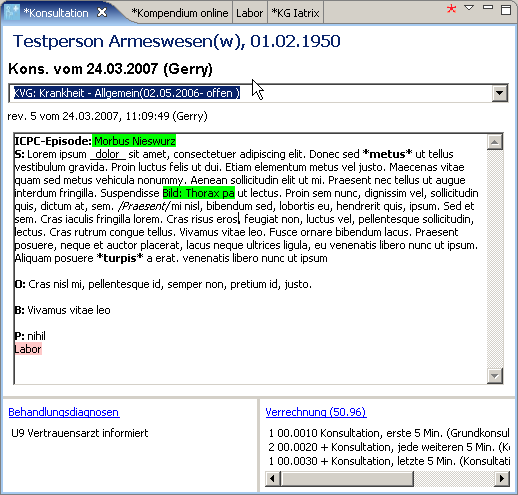
\includegraphics{images/konsview}
  \caption{Konsultation: Detail}
  \label{fig:konsdetail}
\end{center}
\end{figure}

\subsection{AUF}
Diese View dient der Festlegung einer Arbeitsunfähigkeit. (Abb \ref{fig:auf})
\index{AUF} \index{Arbeitsunfähigkeit}. %\usepackage{graphics} is needed for \includegraphics
\begin{figure}[htp]
\begin{center}
  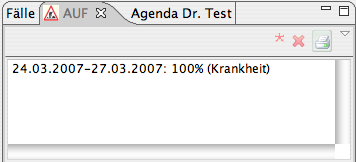
\includegraphics{images/aufview}
  \caption{AUF-View}
  \label{fig:auf}
\end{center}
\end{figure}
Eine AUF bezieht sich immer auf einen bestimmten Fall. Wenn kein Fall markiert
ist, werden Sie aufgefordert, zunächst einen anzugeben.

Wenn Sie auf das \glqq Neu\grqq -Symbol (roter Stern) klicken, erscheint ein
Dialog, in dem Sie Anfang und Ende der neuen Arbeitsunfähigkeit festlegen
können. Klick auf das \glqq Drucker\grqq -Symbol öffnet eine Text-View, in der
Sie noch manuelle Änderungen am AUF-Text ergänzen können, bevor Sie das Zeugnis
definitiv ausdrucken oder aufs Fax senden.

\subsection{Rezepte}
In dieser View werden Rezepte aufgenommen. \index{Rezept}Klicken Sie auf das \glqq Neu\grqq
-Symbol (roter Stern) und es wird ein neues Rezept mit dem Aktuellen Datum
erstellt. Ziehen Sie Artikel mittels Drag\&Drop aus einer Artikelliste oder der
Dauermedikations-View in dieses Rezept. Mit Klick auf das \glqq Drucker\grqq -
Symbol öffnen Sie eine Text-View, in der Sie noch manuelle Änderungen anbringen
können, bevor Sie das Rezept definitiv auf den Drucker oder ein Faxgerät oder in
einen Export-Konnektor senden.
Hierzu muss eine Textvorlage namens \glqq Rezept\grqq
existieren, welche an einer Stelle den Platzhalter [Rezeptzeilen] enthält. Dort
werden die ausgewählten Artikel eingefügt.

\subsection{Heute}
Diese View dient dazu, Konsultationen eines bestimmten Zeitraums (standardmässig
des aktuellen Tages) darzustellen. Sie gibt einen Überblick über Verrechnung und
verrechnete Zeit jeder Konsultation einzeln und der Summe davon, Dies eignet
sich beispielsweise, um abends die Abrechnungen des Tages nachzukontrollieren.


\subsection{Diagnosen}

